
\chapter{Dataset preparation}

\begin{introduction}
In this chapter, it will be discussed various ways of applying artificial intelligence models to archaeology.
\end{introduction}





Deep learning is a subtype of artificial intelligence, which relies on neural networks in order to recognize patterns in the given training data. When trained on a dataset, the network is able to learn many features about it, making it capable of making predictions when presented with new data.


%Two of the pillars of deep learning are the diversity of the dataset, and also the precision of the training annotations. Since the model will be able to learn small possible variations in the data, thus reducing the risk of overfitting, a good dataset is fundamental, even though it is not always possible to obtain a dataset that represents all the input possibilities.

%\subsubsection{Overfitting}
%Overffiting occurs when a model performs very well on training data, yet when presented with new data has trouble making accurate predictions. This can occur for several reasons:
%\begin{itemize}
%\item There is too little training data, creating a dataset that is unrepresentative of all possible inputs.
%
%\item The model is trained for a long time and thus, without an early stop, increasingly makes the itself only an expert on the given type of training data.
%
%\item The model is too complex, causing it to learn not only the necessary predictive features, but also the noise that the inputs may have.
%\end{itemize}

To perform the Odyssey project, the Alto Minho region, in Portugal, was chosen. With the help of the Comunidade Intermunicipal do Alto Minho\cite{comunidadeAltoMinho}, LiDAR data of 2018 was collected, covering 2220 km2, to which later was applied the visualization technique, more specifically LRM. As a result of this process 4 LRM images were generated, corresponding to 4 sub-regions of Alto Minho: Viana do Castelo, Paredes de Coura, Arcos de Valdevez and Parque Nacional da Peneda-Gêrez, having a correspondence of 0.5 meters on the terrain per pixel.
From these 4 sub-regions, the locations of all known tumuli and castros were also provided.

The following table shows the resolution of each image, as well as the number of known annotations and the image size.

\begin{table}[h!]
\centering
\begin{tabular}{|p{3cm}|p{2.5cm}|p{2cm}|p{2cm}|p{2cm}|} 
 \hline
  Region & Resolution(px) & Annotations (tumulis) & Annotations (hillforts) & Size (GB) \\ [0.5ex] 
 \hline\hline
 Viana do Castelo & 19,978x46.000 & 14 & 41 & 3.7\\ 
 Paredes de Coura & 13,999x51,999 & 56 & 65 & 2.9 \\
 Arcos de Valdevez & 15,999x43,999 & 71 & 46 & 2.8\\
 Parque Nacional da Peneda-Gerês & 19,999x44,955 & 135 & 11 & 3.6\\ [1ex] 
 \hline
\end{tabular}
\caption{Description of the dataset used}
\end{table}

The following image shows the joint of the 4 LRM images, corresponding to the entire Alto Minho area where LiDAR data was collected.

\begin{figure}[H]
\centering
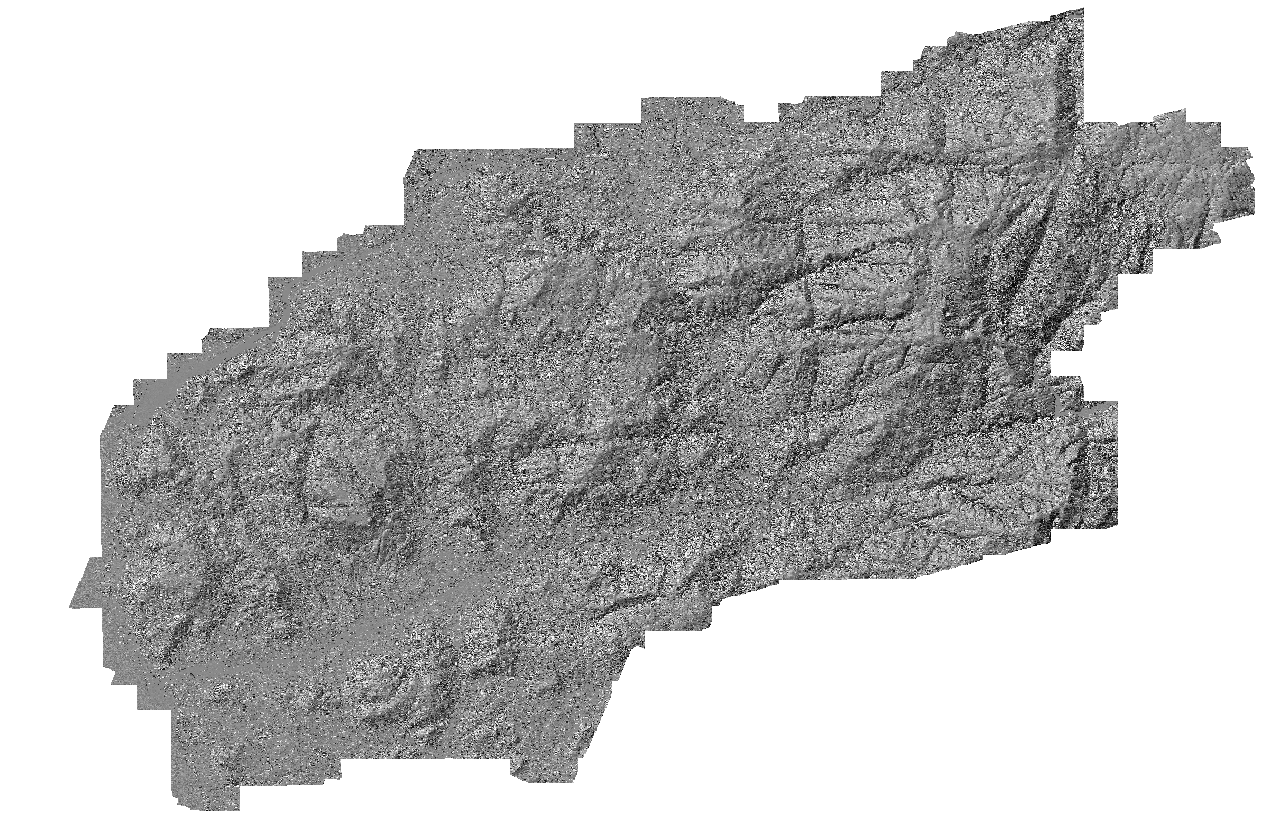
\includegraphics[width=10cm]{images/LRMfinal.png}
\caption{The 4 LRM images together, corresponding to Alto Minho}
\end{figure}
In the two following images, there are two examples of annotations of tumuli on the left side and hillforts on the right side, using the QGUIS software.
\begin{figure}[H]
    \centering
    \subfloat{{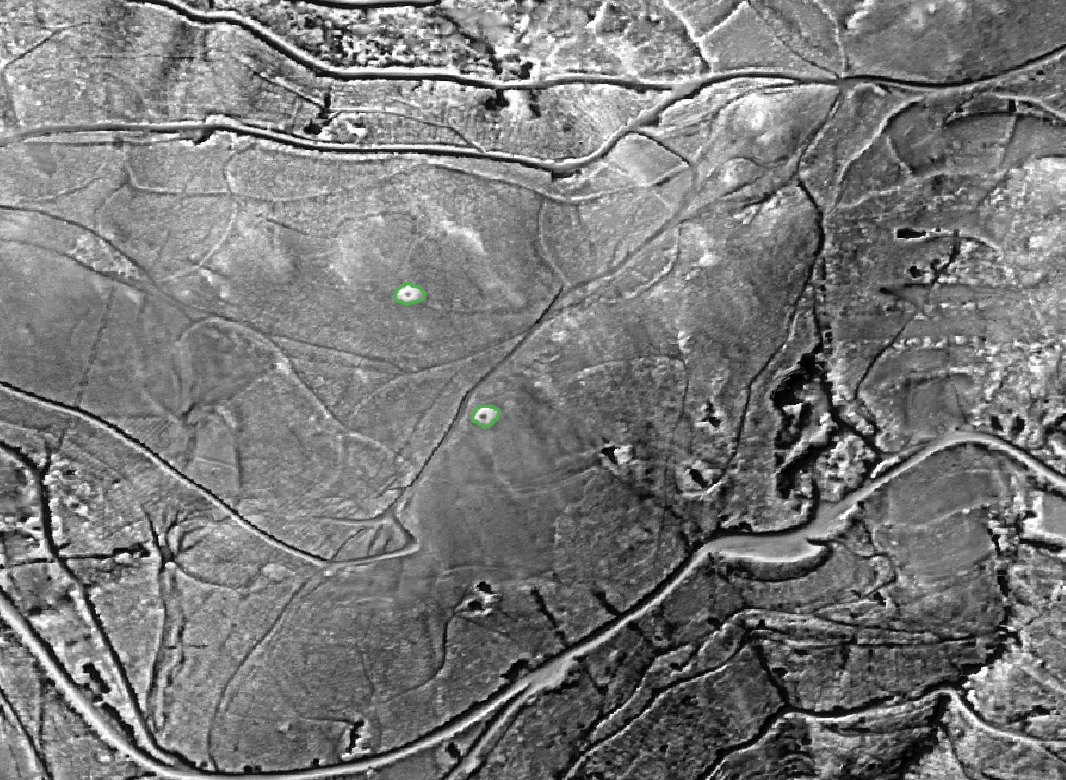
\includegraphics[width=7cm]{images/qgis/qgis2Mamoas.png} }}%
    \qquad
    \subfloat{{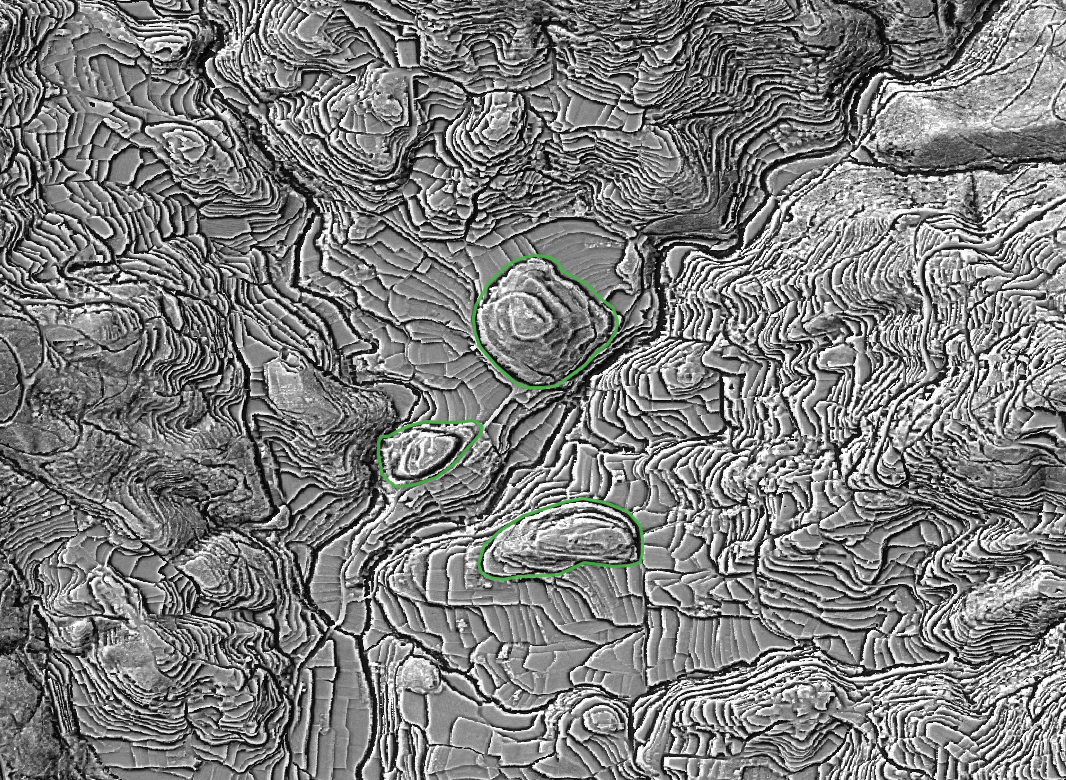
\includegraphics[width=7cm]{images/qgis/qgis3Castros.png} }}%
    \caption{Example of annotations of tumuli on the left side and hillforts on the right side, using QGUIS}%
\end{figure}



%That said, in this project the amount of data provided is relatively small \cite{yolov5recomedacoes}, as you can see, it is recommended to use for each type of object more than 1500 images and more than 10000 annotations to achieve good results. Since YOLOv7 is a relatively large model, this is even more important, due to the possibility of the weights not converge all if the dataset is small, and that is what this section is about, creation of the dataset, as well its augmentation.

\section{Creation of the base dataset}

Along with the images the annotations were also provided in the Well-Know Text (WKT) format. This format indicates in polynomial form the geographical location of the site in question.

However, as it is possible to see from the table above, the 4 LRM images are too large, both for training the YOLOv7 model and the Unet model. Because of this, the 4 images were processed in order to obtain a dataset with 640x640 pixels images, being a typical size to train both YOLOv7 and Unet.

For this, a Python script was used. In this script, one LRM image was loaded at a time, as well as its annotations. To simplify it, separate datasets were generated for the tumuli and for the forts. Then, the annotations were parsed, and using the LRM image metadata, the geographic coordinates of the image extremities were obtained. With that, the coordinates present in the annotation polynomials were converted to pixels using the mapping function, as illustrated below:

\begin{equation}
     pixel = \frac{(coordenate - inMin) * (outMax - outMin)} {(inMax - inMin)} + outMin
     \label{Map function}
\end{equation}

In the function, the inMin and inMax represent the geographic coordinates of the LRM image extremities, whereas the outMin and outMax represent the size of the image in pixels. However, in the y-coordinate, are counted from top to bottom. Therefore, to calculate the y-coordinate of the pixel, outMin and outMax are swapped.

Once this is done, the bounding boxes are stored in a list. The script then iterates over the annotations to create the crops. For each unprocessed annotation, a range of coordinates is generated around the annotation, which will define the region of interest. These coordinates are randomly selected within a specific range around the annotation. The script then checks whether the selected region of interest contains only fully visible objects. If true, the annotations present in the crop are registered as already processed. This is important to maintain the uniqueness of the original dataset annotations. 

The crop is then saved along with the label in YOLO format and a second label containing not the information from the bounding box, but the segmentation. This will be used later for both the Unet and the dataset augmentation.

The script also split the dataset into training and validation, and chose 85\% for training and 15\% for validation.

Finally, the bounding boxes are utilized to store the raw LiDAR data points that correspond to each annotation. These points are saved in separate .las files, with each file containing the points whose coordinates fall within the corresponding bounding box. This approach ensures that the LiDAR data is organized and associated with the specific objects annotated by the bounding boxes.

The use of these files will be explained later.

The next two tables show the results of the dataset creation.

\begin{table}[H]
\centering
\begin{tabular}{|p{3cm}|p{2.5cm}|p{2cm}|} 
\hline
\multicolumn{3}{|c|}{Tumulis} \\
 \hline
  Set & Images & Annotations\\ [0.5ex] 
 \hline
 Training set & 139 & 233 \\ 
 Validation set & 23 & 42  \\[1ex]
 \hline
\end{tabular}
\caption{Tumulis dataset}
\end{table} 

\begin{table}[H]
\centering
\begin{tabular}{|p{3cm}|p{2.5cm}|p{2cm}|} 
\hline
\multicolumn{3}{|c|}{Hillforts} \\
 \hline
  Set & Images & Annotations\\ [0.5ex] 
 \hline
 Training set & 139 & 141 \\ 
 Validation set & 21 & 22  \\[1ex]
 \hline
\end{tabular}
\caption{Hillforts dataset}
\end{table} 


\section{Dataset augmentation}
Deep Learning has revolutionized the field of artificial intelligence, enabling significant advances in areas such as image recognition, natural language processing, and many other complex domains. However, for Deep Learning models to reach their full potential, it is essential to overcome challenges such as sparse training data and limited generalization.

The main reason augmentation is so important is the ability to improve the generalizability of Deep Learning models. With more examples available for training, the model is exposed to a wider variety of cases and patterns, allowing it to learn more robust and variation-resistant features, avoiding overfiting.
Overffiting occurs when a model performs very well on training data, yet when presented with new data has difficulty making correct predictions. This can occur for several reasons\cite{nonmaxsurpression}:
\begin{itemize}
\item There is too little training data, creating a dataset that is unrepresentative of all possible inputs.

\item The model is trained for a long time and thus, without stopping early, increasingly makes the model only an expert on the given type of training data.

\item The model is too complex, causing it to learn not only the necessary predictive features, but also the noise that the inputs may have.

\item The training data contains irrelevant data, called noisy data.
\end{itemize}

This is clearly an undesirable phenomenon.

Analyzing the github repository which contains the code needed to run YOLOv7, is possible to verify that no recommendations for creating a custom dataset are indicated, not even in the published paper \cite{paperyolov7}, in which it is only indicated that the COCO dataset was used to train the model and nothing else is mentioned about datasets. 

However in the YOLOv5 repository, there is a section, where it is given recommendations on how to train a custom dataset, and as said before, it is recommended per object type to have more than 1500 images and more than 10000 annotations \cite{yolov5recomedacoes}, and as it is possible to see, the original dataset is far from containing this amount of data and it was to overcome this problem that two augmentation algorithms were used.
I will refer to the first algorithm as copy paste augmentation and to the second as simple augmentation.

\subsection{Copy paste augmentation}
The augmentation copy paste method used, consists of copying annotated objects and pasting them in areas where it is very certain that there are no unannotated objects.

In the creation of the base dataset, only a small portion of the LRM images were used, leaving a large amount of potential crops with unannotated backgrounds. From here it would be easy to use the segmentation already provided for the archaeological sites, crop and paste in these backgrounds. However, there is one problem, the provided annotations do not result in intensive terrain analysis, leaving the possibility of unannotated sites, which means one cannot If the algorithm crops an image, where there is an unannotated site, this would lead to deterioration of the deep learning algorithm.

It becomes necessary for the copy paste algorithm to be able to discard backgrounds with possible unannotated sites, which is in itself a paradox, since the objective of the project is to detect unannotated sites. To do this we used the yolov5 model trained on the base dataset. This model then becomes responsible for analyzing candidate crops, discarding all those that have possible new sites. 

Since the model was trained on limited data, it is extremely sensitive, so it ends up detecting many shapes that are actually false positives. It is because of this sensitivity that the model is useful in discarding possible crops, and since the background is quite large, even if the model discards many images, the background is not compromised.

A second problem that arises from the copy paste algorithm, is the choice of the paste location. When choosing randomly, it is possible that the archaeological site will be over a river, house, road and so on, which would also lead to a deterioration of the deep learning algorithm. For this reason, the LBR (Local Based Rank) technique was used. This technique consists in classifying the soil areas as subsoil or land-used. For this, the Land-use and Occupation charter of Portugal\cite{charterPortugal} was used. This charter is basically a comprehensive document that provides detailed information about the various types of land use and occupation in Portugal. It serves as a reliable reference for categorizing soil areas into subsoil or land-used regions.

The LBR technique utilizes this charter to determine the classification of soil areas. By referencing the specific guidelines and classifications outlined in the charter, the technique can accurately label each area as either subsoil or land-used, thereby providing valuable context for the augmentation process.

\begin{figure}[H]
\centering
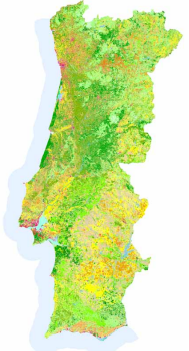
\includegraphics[height=9cm]{images/carta/cartaPortugal.png}
\caption{Land-use and Occupation Charter of Portugal, 2018. Shade of green represent different types of forest, shades of yellow represent different types of agriculture and shades of red represent infrastructures}
\end{figure}

Of the 83 classes present on the chart, only the areas with forest, sparse vegetation and agriculture were kept, and all the others were removed.

In the next two images it is possible to see part of the LRM image of Paredes de Coura, without and with the proposed LBR. The green zones represent the areas of interest, resulted from the charter mentioned.


\begin{figure}[H]
    \centering
    \subfloat{{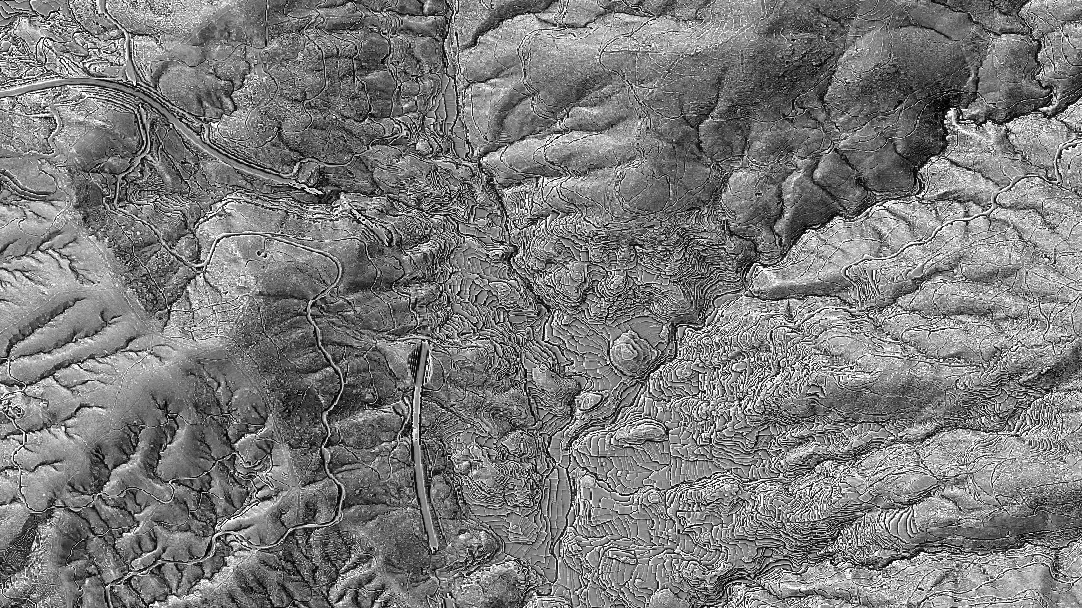
\includegraphics[width=7cm]{images/carta/sem.png} }}%
    \qquad
    \subfloat{{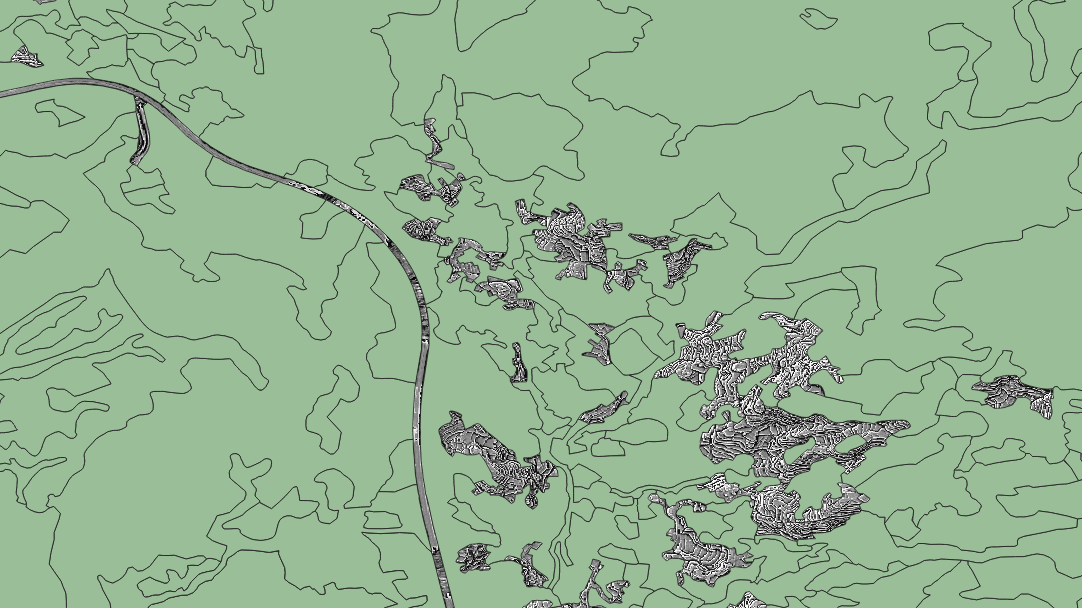
\includegraphics[width=7cm]{images/carta/com.png} }}%
    \caption{Croppred image from Paredes de Coura LRM on the left, and the same image with the LBR on the right}%
\end{figure}

Using these two methods, the dataset was then created, it is worth mentioning that before pasting the annotation, one of the following geometric transformations was applied: flip left to right, flip top to bottom, rotate 90, 180 or 270 degrees and transpose. For each annotation a transformation was randomly selected selectively and then applied.

Additionally, 10\% background was added, following yolov5's recommendations.

Along with the respective labels for the yolo, labels with the segmentation were also saved, which will be used later in Unet.

For the tumuli, being a relatively small object, it was chosen to add 8 tumulis per image, for the castros, being larger objects, it was chosen to add 5 hillforts per image.

In the following two images, there are two examples of the copy paste augmentation, on the left side tumuli and on the right side hillforts.
\begin{figure}[H]
    \centering
    \subfloat{{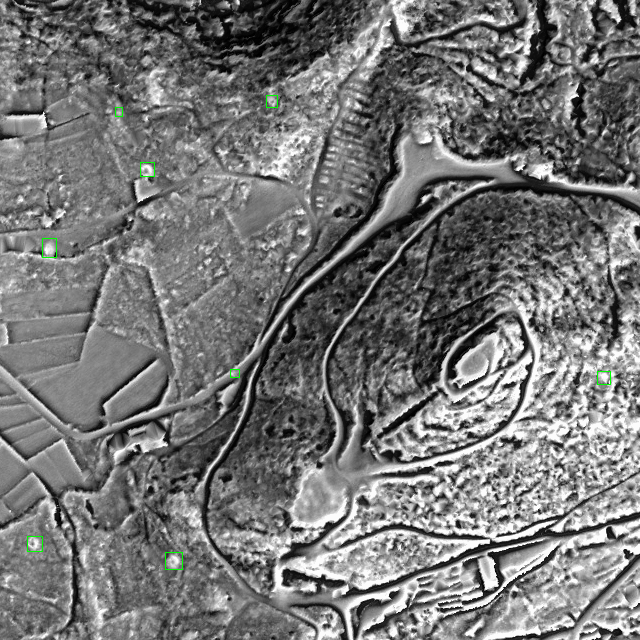
\includegraphics[width=7cm]{images/datasetExemples/aug/mamoas_aug_example.png} }}%
    \qquad
    \subfloat{{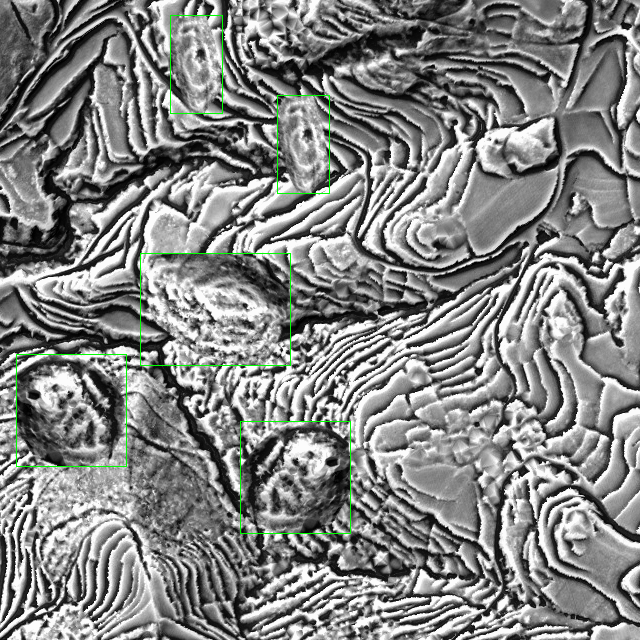
\includegraphics[width=7cm]{images/datasetExemples/aug/castros_aug_example.png} }}%
    \caption{Examples of copy paste augmentation}%
\end{figure}

The two following tables contain the results from copy paste augmentation.

\begin{table}[H]
\centering
\begin{tabular}{|p{3cm}|p{2.5cm}|p{2cm}|} 
\hline
\multicolumn{3}{|c|}{Tumulis} \\
 \hline
  Set & Images & Annotations\\ [0.5ex] 
 \hline
 Training set & 2363 & 15787 \\ 
 Validation set & 391 & 2611  \\[1ex]
 \hline
\end{tabular}
\caption{Tumulis copy paste dataset}
\end{table} 

\begin{table}[H]
\centering
\begin{tabular}{|p{3cm}|p{2.5cm}|p{2cm}|} 
\hline
\multicolumn{3}{|c|}{Hillforts} \\
 \hline
  Set & Images & Annotations\\ [0.5ex] 
 \hline
 Training set & 2304 & 9668 \\ 
 Validation set & 256 & 1071  \\[1ex]
 \hline
\end{tabular}
\caption{Hillforts copy paste dataset}
\end{table} 


\subsection{Simple augmentation}
The second augmentation algorithm, referred to as simple augmentation, is a much more straightforward approach compared to the first one. It involves centering each object within a 640x640 pixel box and randomly shifting the box. Subsequently, the algorithm verifies if the object, along with other nearby objects, remains completely inside the box. If all the objects are contained within the box, a similar transformation to the previous algorithm is applied, not to the individual object but to the entire image. Finally, the modified images and their corresponding labels are saved.

This method was applied several times for the same annotation enabling the generation of annotated data that retains the same objects but positions them differently within the image, resulting in varied backgrounds.

The next images show examples of the same annotation but on different images resulting from the augmentation.

\begin{figure}[H]
    \centering
    \subfloat{{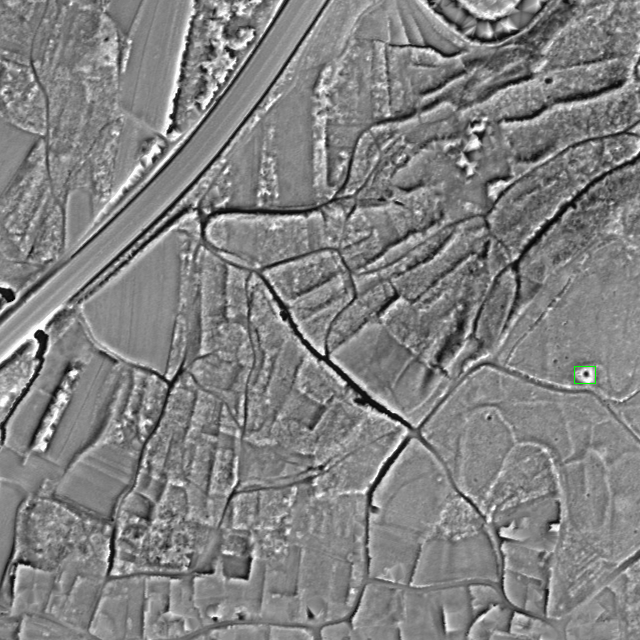
\includegraphics[width=7cm]{images/datasetExemples/maia/mamoas1.png} }}%
    \qquad
    \subfloat{{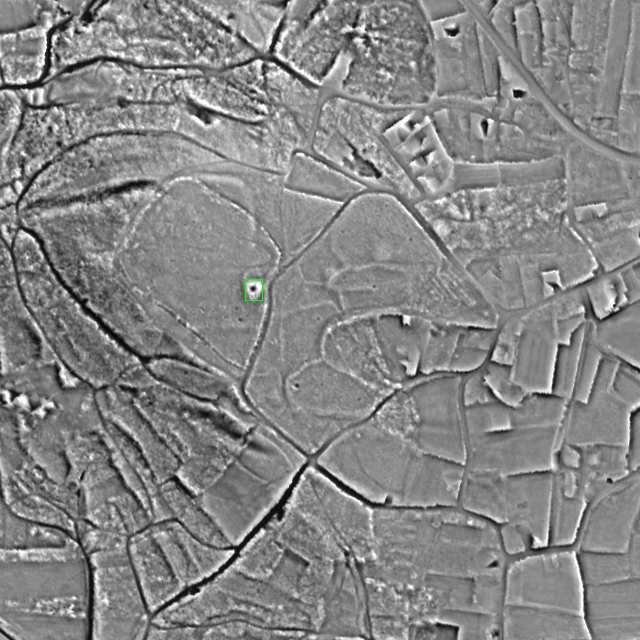
\includegraphics[width=7cm]{images/datasetExemples/maia/mamoas2.png} }}%
    \caption{Example of the same tumuli but in different position of the image}%
\end{figure}

\begin{figure}[H]
    \centering
    \subfloat{{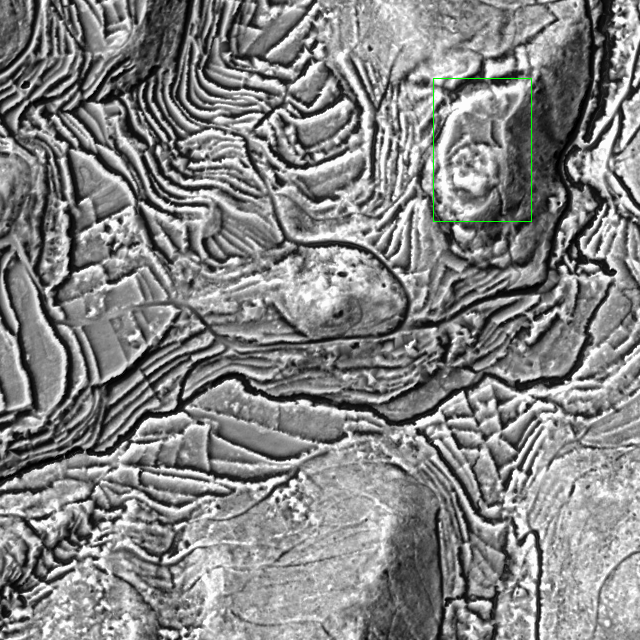
\includegraphics[width=7cm]{images/datasetExemples/maia/castros1.png} }}%
    \qquad
    \subfloat{{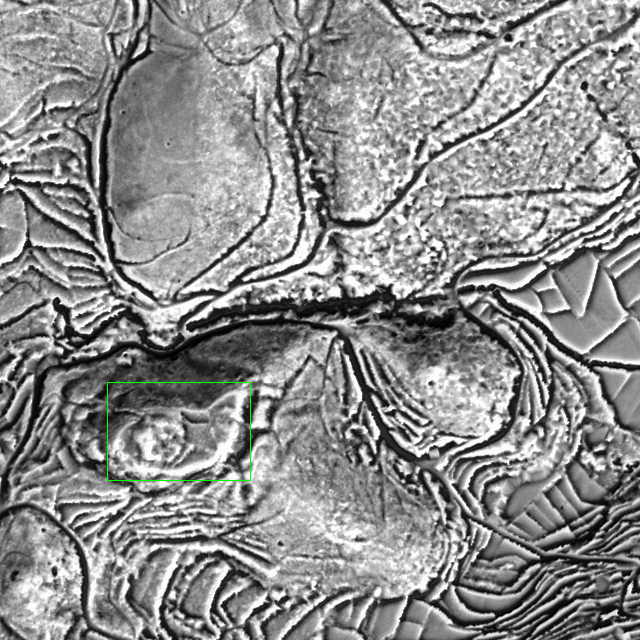
\includegraphics[width=7cm]{images/datasetExemples/maia/castros2.png} }}%
    \caption{Example of the same hillforts but in different position of the image}%
\end{figure}

The next two tables show the results of the dataset creation.

\begin{table}[H]
\centering
\begin{tabular}{|p{3cm}|p{2.5cm}|p{2cm}|} 
\hline
\multicolumn{3}{|c|}{Tumulis} \\
 \hline
  Set & Images & Annotations\\ [0.5ex] 
 \hline
 Training set & 1171 & 2658 \\ 
 Validation set & 209 & 466  \\[1ex]
 \hline
\end{tabular}
\caption{Tumulis simple dataset}
\end{table} 

\begin{table}[H]
\centering
\begin{tabular}{|p{3cm}|p{2.5cm}|p{2cm}|} 
\hline
\multicolumn{3}{|c|}{Hillforts} \\
 \hline
  Set & Images & Annotations\\ [0.5ex] 
 \hline
 Training set & 691 & 716 \\ 
 Validation set & 124 & 128  \\[1ex]
 \hline
\end{tabular}
\caption{Hillforts simple dataset}
\end{table} 